\documentclass[9pt,landscape]{article}
\usepackage{{./../static/style}}
\pdfinfo{
  /Title (PyAnsys cheat sheet)
  /Creator (TeX)
  /Producer (pdfTeX 1.40.0)
  /Author (Ansys)
  /Subject (PyAnsys)
  /Keywords (PyAnsys, PyFluent, cheat sheet, template)}

\begin{document}
\raggedright
\footnotesize

% Add the title of cheat sheet here
% ----------------------------------------
\begin{center}
     \Huge{\textbf{PyFluent cheat sheet}} \\
\end{center}
\begin{center}
     \Large{\textbf{Solver settings object interface}} \\
     \small{\textbf{Version: 0.13 (stable)}} \\
\end{center}

\AddToShipoutPicture*
  {\put(670,577.5){
\includegraphics[height = 1.2cm]{ansys.png}}}
\AddToShipoutPictureBG*{
\includegraphics[width=\paperwidth]{bground.png}}
\vspace{-0.15cm}
\noindent\makebox[\linewidth]{\rule{\paperwidth}{2pt}}

\begin{multicols}{3}
\setlength{\premulticols}{1pt}
\setlength{\postmulticols}{1pt}
\setlength{\multicolsep}{1pt}
\setlength{\columnsep}{2pt}

% session starts here. 
% First colomn
% --------------------------------------------------------------------------------
\vfill

\section{
\includegraphics[height=\fontcharht\font`\S]{slash.png} Launch Fluent locally} 
\pythoncode{scripts/generated_scripts/pyfluent_script_0.py}

\section{
\includegraphics[height=\fontcharht\font`\S]{slash.png} Import mesh in launched session}

Read the available mesh file in the Fluent session:

\pythoncode{scripts/generated_scripts/pyfluent_script_1.py}

Use specific methods to read case files and case data files:

\pythoncode{scripts/generated_scripts/pyfluent_script_2.py}


\section{
\includegraphics[height=\fontcharht\font`\S]{slash.png} Enable heat transfer physics}

Enable heat transfer by activating the energy equation:

\pythoncode{scripts/generated_scripts/pyfluent_script_3.py}

\section{
\includegraphics[height=\fontcharht\font`\S]{slash.png} Access the object state using \texttt{pprint}}

\pythoncode{scripts/generated_scripts/pyfluent_script_4.py}

\section{
\includegraphics[height=\fontcharht\font`\S]{slash.png}  Define materials}
Use \texttt{solver} settings objects to define materials:
\pythoncode{scripts/generated_scripts/pyfluent_script_5.py}

% Second column
% --------------------------------------------------------------------------------
% row 1 col 2
\vfill

% row 2 col 2
\section{
\includegraphics[height=\fontcharht\font`\S]{slash.png}  Define boundary conditions}

Use \texttt{solver} settings objects to define boundary conditions:
\pythoncode{scripts/generated_scripts/pyfluent_script_6.py}


\section{
\includegraphics[height=\fontcharht\font`\S]{slash.png}  Modify cell zone conditions} 
Use \texttt{solver} settings objects to modify cell zone conditions.
\pythoncode{scripts/generated_scripts/pyfluent_script_7.py}


% Third column
% --------------------------------------------------------------------------------
\vfill
% row 1 col 3

\section{
\includegraphics[height=\fontcharht\font`\S]{slash.png}  Apply solution settings}
Use \texttt{solver} settings objects to apply solution settings, initialize, and solve.

\pythoncode{scripts/generated_scripts/pyfluent_script_8.py}

% row 2 col 3
\section{
\includegraphics[height=\fontcharht\font`\S]{slash.png}  Postprocessing}
Postprocess data with the \texttt{results} object. For example, create and display contours on a plane:

\pythoncode{scripts/generated_scripts/pyfluent_script_9.py}
\section{
\includegraphics[height=\fontcharht\font`\S]{slash.png}  Temperature contour}
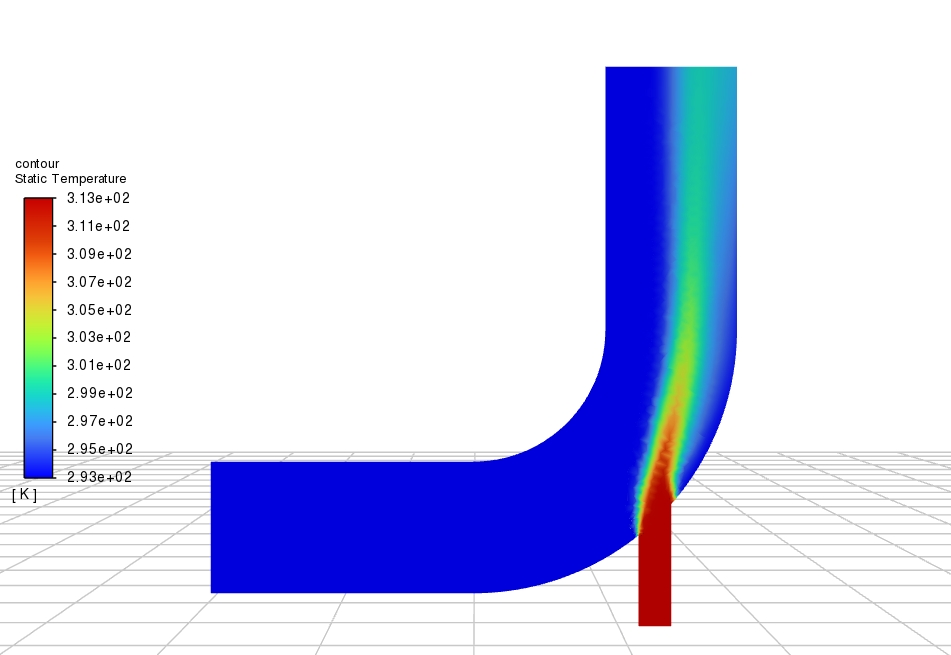
\includegraphics[scale=0.15]{mixing_elbow_pyfluent.jpg}
\centering

% Add subsection
% This section includes useful links to the documentation.
% Examples: installation, API reference, commands, examples.
% Replace 'name of link' with appropriate display text.

\subsection{References from PyFluent documentation}
\begin{itemize}
\item \href{https://fluent.docs.pyansys.com/version/stable/getting_started/index.html}{\color{blue}{Getting started}}  
\item \href{https://fluent.docs.pyansys.com/version/stable/api/solver/settings.html#ref-settings}{\color{blue}{Solver settings objects}}
\item \href{https://fluent.docs.pyansys.com/version/stable/examples/index.html}{\color{blue}{Examples}}
\end{itemize}
\end{multicols}

% Footer session of the latex with link to documentation and GitHub page
\vspace{-0.15cm}
\noindent\makebox[\linewidth]{\rule{\paperwidth}{4pt}}
\begin{center}
Getting started with PyFluent 
\includegraphics[height=\fontcharht\font`\S]{slash.png} \href{https://github.com/ansys/pyfluent}{\color{blue}{PyFluent on GitHub}}} 
\includegraphics[height=\fontcharht\font`\S]{slash.png} Visit \code{\href{https://fluent.docs.pyansys.com/}}{\color{blue}{fluent.docs.pyansys.com}}
\end{center}
\end{document}
